\section{Problem 4 - Regression}
\subsection{a)}
Using the euclidean distance I get an RSME value of

$$RMSE = 0.82430$$

\begin{figure}[H]
    \centering
    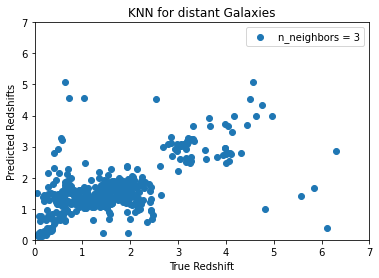
\includegraphics[width=0.75\textwidth]{Figures/Q4_a_galaxiesPlot.png}
    \caption{Plot of kNN with k = 3}
\end{figure}


\subsection{b)}
Using the other distance calculation as given in the exam set I get the following RSME value
$$RMSE = 1.100519$$
\begin{figure}[H]
    \centering
    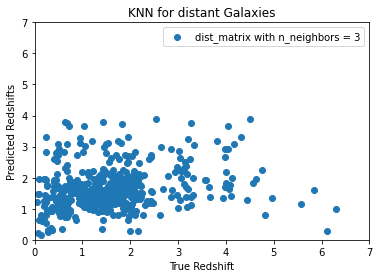
\includegraphics[width=0.75\textwidth]{Figures/Q4_b_wMatrix_plot.png}
    \caption{Plot of kNN with k = 3 and distance matrix}
\end{figure}

My assumption is, that the distance matrix will lower/lessen the influence of all 
the features/attributes except for the last two, since they are set to 1.0.
\subsection{c)}